\documentclass[11pt]{article}
\usepackage{../cs170}

\def\title{Homework 12}
\def\duedate{Monday 11/20/2023, at 10:00 pm (grace period until 11:59pm)}

\begin{document}
\maketitle


Due \textbf{\duedate}

\question{Study Group}
List the names and SIDs of the members in your study group.
If you have no collaborators, you must explicitly write ``none''.

\begin{solution}
	None in particular. Got a bit of guidance on problem 4 by TAs.   
\end{solution}

\question{Vertex Cover to Set Cover}

To help jog your memory, here are some definitions:

\begin{quote}
\textbf{Vertex Cover:} given an undirected unweighted graph $G = (V, E)$, a vertex cover $C_V$ of $G$ is a subset of vertices such that for every edge $e=(u, v) \in E$, at least one of $u$ or $v$ must be in the vertex cover $C_V$.

\textbf{Set Cover:} given a universe of elements $U$ and a collection of sets $\mathcal{S} = \{S_1, \dots, S_m\}$, a set cover is any (sub)collection $C_S$  whose union equals $U$.

In the \textit{minimum vertex cover problem}, we are given an undirected unweighted graph $G = (V,E)$, and are asked to find the smallest vertex cover. 
For example, in the following graph,  $\{A, E, C, D\}$ is a vertex cover,  but not a minimum vertex cover.
The minimum vertex covers are $\{B, E, C\}$ and $\{ A, E, C\}$. \vskip 0.5cm
\begin{center}

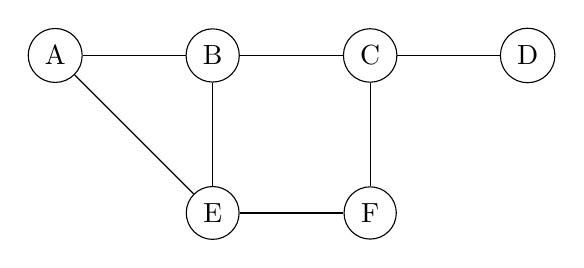
\begin{tikzpicture}
[ar/.style={thick},no/.style={draw,circle}]
\node [no] at (0cm,2cm) (A) {A};
\node [no] at (2cm,2cm) (B) {B};
\node [no] at (4cm,2cm) (C) {C};
\node [no] at (6cm,2cm) (D) {D};
\node [no] at (2cm,0cm) (E) {E};
\node [no] at (4cm,0cm) (F) {F};

\draw (A) -- node  {}(B);
\draw (A) -- node  {}(E);
\draw (B) -- node  {}(C);
\draw (B) -- node  {}(E);
\draw (E) -- node  {}(F);
\draw (C) -- node  {}(F);
\draw (C) -- node  {}(D);
\end{tikzpicture}
\end{center}

Then, recall in the \textit{minimum set cover problem}, we are given a set $U$ and a collection $\mathcal{S} = \{S_1, \ldots, S_m\}$ of subsets of $U$, and are asked to find the smallest set cover.
For example, given $U := \{ a, b, c, d \}$, $S_1 := \{a, b, c\}$, $S_2 := \{ b, c\}$,  and $S_3 := \{ c, d \} $, a solution to the problem is $C_S = \{S_1, S_3\}$.
\end{quote}

\textbf{Give an efficient reduction from the minimum vertex cover problem to the minimum set cover problem. Briefly justify the correctness of your reduction (i.e. 1-2 sentences).}

\begin{solution}
	\textbf{So it turns out that this is the same problem as homework 10 problem 7. I took inspiration from the 
		official solution, but wrote it in my own language and made sure I understood the solution properly 
	before typing up my own solution.}

	We can create a set cover instance where for every vertex \( v \), its set consists of \( v \) and all 
	vertices connected to \( v \). In other words, first label the vertices \( v_1, v_2, \dots, v_n \), and 
	have the sets \( S_i \) contain \( v_i \) and all vertices that share an edge with \( v_i \).
	
	Then, once the set cover instance is solved, the indices of the sets that it chooses in \( C_S \) will be 
	the minimum vertex cover (in other words, if \( C_S = \{S_1, S_2, S_3\}  \), then our vertex cover is 
	\( C_V = \{v_1, v_2, v_3\}  \).

	\textbf{Proof of Correctness:} Based on the way we constructed our sets, each set chosen in our set cover 
	corresponds directly to the vertex that would be chosen for a vertex cover. In other words, the set cover 
	we choose will also be a vertex cover. 

	To prove this, consider a given set cover \( C_S \), and its corresponding vertex cover \( C_V \). Suppose 
	there is an edge \( (u, v) \) that isn't covered by \( C_V \). This implies that both vertices \( u, v \) did
	not exist within the vertex cover, but this is impossible, since this would imply that \( C_S \) was not 
	a valid set cover (as a set cover covers all vertices). Hence, each set cover corresponds to some vertex
	cover. Therefore, the minimum set 
	cover also corresponds directly to the minimum vertex cover, as desired. 
\end{solution}

\newpage

\question{Reduction to 3-Coloring}

Given a graph $G = (V, E)$, a valid 3-coloring assigns each vertex in the graph a color from \{red, green, blue\} such that for any edge $(u, v)$, $u$ and $v$ have different colors. In the 3-coloring problem, our goal is to find a valid 3-coloring if one exists. In this problem, we will give a reduction from 3-SAT to the 3-coloring problem. Since we know that 3-SAT is NP-Hard (there is a reduction to 3-SAT from every NP problem), this will show that 3-coloring is NP-Hard (there is a reduction to 3-coloring from every NP problem).

\noindent In our reduction, the graph will start with three special vertices, labelled $v_{\textsf{TRUE}}$, $v_{\textsf{FALSE}}$, and $v_{\textsf{BASE}}$, as well as the edges $(v_{\textsf{TRUE}}, v_{\textsf{FALSE}})$, $(v_{\textsf{TRUE}}, v_{\textsf{BASE}})$, and $(v_{\textsf{FALSE}}, v_{\textsf{BASE}})$. 
\begin{subparts}

\subpart For each variable $x_i$ in a 3-SAT formula, we will create a
pair of vertices labeled $x_i$ and $\lnot x_i$. How should we add
edges to the graph such that in any valid 3-coloring, one of
$x_i, \lnot x_i$ is assigned the same color as $v_{\textsf{TRUE}}$ and the other is assigned the same color as $v_{\textsf{FALSE}}$? 

\textit{Hint: any vertex adjacent to $v_{\textsf{BASE}}$ must have the same color as either $v_{\textsf{TRUE}}$ or $v_{\textsf{FALSE}}$. Why is this?}

\begin{solution}
	I'll assign \( x_i \) to \( v_\textsf{TRUE} \) and \( \neg x_i \) to \( v_{\textsf{FALSE}} \). We can do 
	this by connecting \( x_i \) to \( v_{\textsf{BASE}} \) and \( v_{\textsf{FALSE}} \), and 
	\( \neg x_i  \) to \( v_{\textsf{BASE}} \) and \( v_{\textsf{TRUE}} \). This way, \( x_i \) doesn't share 
	the same color as \( v_{\textsf{BASE}} \) or \( v_{\textsf{FALSE}} \), and since we only have 3 colors, 
	it must then share the same color as \( v_{\textsf{TRUE}} \). A similar approach shows that \( \neg x_i \) 
	must have the same color as \( v_{\textsf{FALSE}} \). 
\end{solution}

\subpart Consider the following graph, which we will call a ``gadget'':

\begin{center}
\begin{tikzpicture}[
node distance =6mm and 12mm,
C/.style = {circle, draw, minimum size=1em}
                    ] 
\node[fill=gray!40] (v1) [C] {$v_1$};
\node (v2) [C, above right=of v1] {$v_2$};
\node (v3) [C, below right=of v1] {$v_3$};
\node (v4) [C, right=of v2] {$v_4$};
\node (v5) [C, above right=of v4] {$v_5$};
\node (v6) [C, below right=of v4] {$v_6$};
\node[fill=gray!40] (v7) [C, right=of v5] {$v_7$};
\node[fill=gray!40] (v8) [C, right=of v6] {$v_8$};
\node[fill=gray!40] (v9) [C, right=4.85cm of v3] {$v_9$};

\draw (v1) -- (v2);
\draw (v1) -- (v3);
\draw (v2) -- (v3);
\draw (v2) -- (v4);
\draw (v3) -- (v9);
\draw (v4) -- (v5);
\draw (v4) -- (v6);
\draw (v5) -- (v7);
\draw (v5) -- (v6);
\draw (v6) -- (v8);
    \end{tikzpicture}
    \end{center}

Consider any valid 3-coloring of this graph that does \textit{not} assign the color blue to any of the gray vertices ($v_1, v_7, v_8, v_9)$. Show that if $v_1$ is assigned the color green, then at least one of $\{v_7, v_8, v_9\}$ is assigned the color green.

\textit{Hint: it's easier to prove the contrapositive!}

\begin{solution}
	The contrapositive statement is that if none of \( v_7, v_8, v_9 \) are colored green, then \( v_1 \) is 
	also not colored green. Given this statement, we'll work backwards from \( v_7, v_8, v_9 \). Because
	\( v_7, v_8, v_9 \) cannot be colored blue, then they must be colored red. The following 
	is a valid coloring of the graph in this case:

	\begin{center}
	\begin{tikzpicture}[
		node distance =6mm and 12mm,
		C/.style = {circle, draw, minimum size=1em}
							] 
		\node[fill=red!40] (v1) [C] {$v_1$};
		\node[fill=blue!40] (v2) [C, above right=of v1] {$v_2$};
		\node[fill=green!40] (v3) [C, below right=of v1] {$v_3$};
		\node[fill=red!40] (v4) [C, right=of v2] {$v_4$};
		\node[fill=blue!40] (v5) [C, above right=of v4] {$v_5$};
		\node[fill=green!40] (v6) [C, below right=of v4] {$v_6$};
		\node[fill=red!40] (v7) [C, right=of v5] {$v_7$};
		\node[fill=red!40] (v8) [C, right=of v6] {$v_8$};
		\node[fill=red!40] (v9) [C, right=4.85cm of v3] {$v_9$};

		\draw (v1) -- (v2);
		\draw (v1) -- (v3);
		\draw (v2) -- (v3);
		\draw (v2) -- (v4);
		\draw (v3) -- (v9);
		\draw (v4) -- (v5);
		\draw (v4) -- (v6);
		\draw (v5) -- (v7);
		\draw (v5) -- (v6);
		\draw (v6) -- (v8);
		\end{tikzpicture}
	\end{center}
	Alternatively, one could also swap the green and blue colors around, but that doesn't change the overall 
	coloring of the graph (you could just swap all greens and blues here the coloring would still be valid).

	This is also an exhaustive list of possible colorings: \( v_6 \) and \( v_5 \) are forced to be 
	green and blue because \( v_7 \) and \( v_8 \) are red, which forces \( v_4  \) to also be red. This then 
	forces \( v_2  \) to be either green or blue. On the other hand, because  \( v_9 \) is red, this also forces 
	\( v_3  \) to be green or blue. WLOG if \( v_2  \) is blue, this means that \( v_3 \) is green, forcing 
	\( v_1 \) to be red. 
\end{solution}

\subpart We have now observed the following about the graph we are creating in the reduction:
\begin{enumerate}[(i)]
\item For any vertex, if we have the edges $(v, v_{\textsf{FALSE}})$ and $(v, v_{\textsf{BASE}})$ in the graph, then in any valid 3-coloring $v$ will be assigned the same color as $v_{\textsf{TRUE}}$. 

\item Through brute force one can also show that in a gadget, if all the following hold:
\begin{enumerate}[(1)]
\item All gray vertices are assigned the color red or green.
\item $v_1$ is assigned the color green.
\item At least one of $\{v_7, v_8, v_9\}$ is assigned the color green.
\end{enumerate}
Then there is a valid coloring for the white vertices in the gadget. 
\end{enumerate}

Using these observations and your answers to the previous parts, \textbf{give
a reduction from 3-SAT to 3-coloring. Prove that your reduction is correct (you do not need to prove any of the observations above). }

\emph{Hint: create a new gadget per clause!}

\begin{solution}
	For each clause, we will create a new gadget, and let \( v_7, v_8, v_9 \) represent the literals in 
	that clause. 
	Then, 
	depending on their identity (whether the variable is \( x_{i} \) or \( \neg x_{i} \) ), then we connect them 
	in the way described in part (a). This way, all literals \( x_i \) are the same color, and \( \neg x_i \) as 
	well. 

	Further, we will connect all instances of \( v_1 \) to \( v_{\textsf{BASE}} \) and \( v_{\textsf{FALSE}} \), 
	so they have the same color as \( v_{\textsf{TRUE}} \). If there is a valid coloring on this 
	graph, then we know that this 3-SAT instance has a satisfying assignment. 

	\textbf{Proof of Correctness:} If this is a valid 3-coloring instance, then we know that each 
	instance of \( v_1 \) is colored the same as \( v_{\textsf{TRUE}} \). Then, since the literals \( x_i \) 
	(corresponding to \( v_7, v_8, v_9 \)) are colored either  
	\( v_{\textsf{TRUE}} \) or \( v_{\textsf{FALSE}} \), then we know that one of them must be colored 
	the same as \( v_1 \), or \( v_{\textsf{TRUE}} \). The coloring of the literals can then be interpreted
	as the assignment of literals \( x_i \) that satisfies the 3-SAT instance (those that have the same color 
	as \( v_{\textsf{TRUE}} \) are the literals that need to be set to true to satisfy 3-SAT).
\end{solution}

\end{subparts}

\newpage

\question{$k$-XOR}

In the $k$-XOR problem, we are given $n$ boolean variables $x_1, x_2, \ldots, x_n$, a list of $m$ clauses each of which is the XOR of exactly $k$ distinct variables (that is, the clause is true if and only if an odd number of the $k$ variables in the clause are true), and an integer $r$. Our goal is to decide if there is some assignment of variables that satisfies at least $r$ clauses.

\begin{subparts}
\subpart In the Max-Cut problem, we are given an undirected unweighted graph $G=(V, E)$ and integer $c$ and want to find a cut $S \subseteq V$ such that at least $c$ edges cross this cut (i.e. have exactly one endpoint in $S$). Give and argue correctness of a reduction from Max-Cut to $2$-XOR.

\textit{Hint: every clause in 2-XOR is equivalent to an edge in Max-Cut.}

\begin{solution}
	Following the hint, we can construct a graph using the literals \( x_i \) such that for every clause 
	\( x_i \oplus x_j \) (\( \oplus \) is the symbol for XOR apparently), there exists an edge between 
	\( x_i \) and \( x_j \). Then, we can set \( c = r \) 
	and find a max-cut on this graph. 

	If a max-cut is found, then we know that \( r \) edges cross the cut. Then, we can set all the variables 
	on one side of the cut to be true, which satisfies \( r \) clauses, so we're done. 
\end{solution}

\subpart Give and argue correctness of a reduction from $3$-XOR to $4$-XOR.

\begin{solution}
	The key to this problem is to notice that the condition for satisfying 3-XOR is actually the same as 
	4-XOR, in the sense that the number of literals that are set to true in each clause is the same.

	Given a 3-XOR instance, we can convert this into a 4-XOR instance by adding a dummy variable to every clause. 
	Then, we solve the 4-XOR instance. To recover back to the 3-XOR instance, we check whether the dummy 
	variables in each clause were set to true or false. 

	\textit{Case 1:} If the dummy variable is set to true, then check if any other variable in that clause 
	is set to true. If yes, then this clause is fine in the 3-XOR instance. Otherwise, this clause will fail 
	the 3-XOR instance. 

	\textit{Case 2:} If the dummy variable is set to false, we don't really care about it -- it means that 
	the clause was satisfied without the need of the dummy variable, so it will also be satisfied in the 3-XOR
	instance. 
\end{solution}
\end{subparts}

\newpage

\question{Dominating Set (Optional)}

A dominating set of a graph $G = (V, E)$ is a subset $D$ of $V$, such that
every vertex not in $D$ is a neighbor of at least one vertex in
$D$. Let the Minimum Dominating Set problem be the task of determining
whether there is a dominating set of size $\leq k$. Show that the Minimum Dominating Set problem is NP-Complete. You may
assume that $G$ is connected.

\textit{Hint: Try reducing from Vertex Cover or Set Cover.}

\newpage

\question{Orthogonal Vectors (Optional)}
In the 3-SAT problem, we have $n$ variables and $m$ clauses, where each clause is the OR of (at most) three of these variables or their negations. The goal of the problem is to find an assignment of variables that satisfies all the clauses, or correctly declare that none exists.

\noindent In the orthogonal vectors problem, we have two sets of vectors $A, B$. All vectors are in $\{0, 1\}^m$, and $|A|=|B|=n$. The goal of the problem is to find two vectors $a \in A, b \in B$ whose dot product is 0, or correctly declare that none exists. The brute-force solution to this problem takes $O(n^2 m)$ time: We compute all $|A||B| = n^2$ dot products between two vectors in $A, B$, and each dot product takes $O(m)$ time.

\noindent Show that if there is a $O(n^c m)$-time algorithm for the orthogonal vectors problem for some $c \in [1, 2)$, then there is a $O(2^{cn/2} m)$-time algorithm for the 3-SAT problem. For simplicity, you may assume in 3-SAT that the number of variables must be even. 

\noindent \textit{Hint: Try splitting the variables in the 3-SAT problem into two groups.}

\end{document}

